\section{Integrating external sources of information}

\subsection{Sources of information}

Currently CERN runs three PhEDEx instances:

\begin{description}
	\item[Production] is used for production CMS data transfers
	\item[Debug] is used for link monitoring and link commissioning tests
	\item[Development] is used for testing software and DB schema upgrades
\end{description}

Although the instances run on the same infrastructure, each one is independent 
of the rest. The Production instance chooses transfer sources based on its 
internal monitoring data alone. The Debug instance, on the other hand,
has monitoring information about many more links. Because of this, it makes
sense that where links are shared, network statistics should be shared
as well (Figure \ref{fig:Prod-vs-Debug})

\begin{figure}[h]
  \centering
  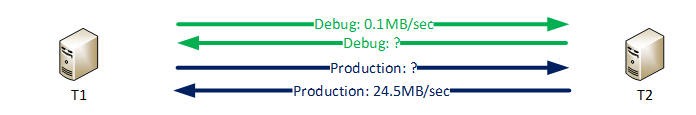
\includegraphics[width=0.95\textwidth]{Figures/Debug-vs-Prod-instance.png}
  \caption{Example case where the Production and Debug instances contain complementary
  data}
  \label{fig:Prod-vs-Debug}
\end{figure} 

A tool has been developed which retrieves statistics from all instances and 
aggregates the data. This tool then produces a file that the FileRouter agent
can use to supplement its internal statistics, giving it a more complete overview of the
network performance.

The next step is to integrate it with perfSONAR\cite{perfSONAR}, effectively gaining a 
more comprehensive picture of what's happening on the network. At the time of
writing this paper, perfSONAR is yet to be deployed on all WLCG sites. We also
lack a perfSONAR API which we can call to retrieve this data. Finally, PhEDEx will need
some work to use this data, since it has its own internal naming convention for sites which corresponds to their logical identity, rather than to their internet hostnames.
